	\documentclass[preprint,11pt,authoryear]{elsarticle}
	\usepackage{amsmath}
	\usepackage[font=sf, labelfont={sf,bf}, margin=0cm]{caption}
	\usepackage[inline]{enumitem}
	\usepackage{epstopdf}   
	\usepackage[margin=1in]{geometry}
	\usepackage{lineno}
	\usepackage{placeins}
	\usepackage{subcaption}
	\usepackage{color}
	\usepackage{algorithm}
	\usepackage{algpseudocode}
	%\usepackage[section]{placeins} %prevents floats from appearing before their sections. web address  https://tex.stackexchange.com/questions/32598/force-latex-image-to-appear-in-the-section-in-which-its-declared
	\usepackage{float}
	
	\journal{Chemical Engineering Research and Design}
	\begin{document}
	\begin{frontmatter}
	\title{ NSF CDSE DRAFT 02}
	\author{Thor }
	\author{Gibbs }
	\author{Zeus }
	\author{the guy who invented sticky notes }
	\author{Santa Claus\corref{cor1}} 
	\ead{santaclaus}
	\cortext[cor1]{Corresponding author}
	\address{North Pole department of ice and snow Fwding address - Department of Chemical and Biochemical Engineering, Rutgers, The State University of New Jersey, Piscataway, NJ, USA 08854}
	\begin{abstract}
	 abstract text goes here ...
	\end{abstract}
	\begin{keyword}
	Population balance model \sep heteroaggregation \sep alginate  \sep chitosan \sep oppositely charged
	\end{keyword}
	\end{frontmatter}
	\linenumbers
	
	\section{Introduction \& Objectives} 
	description of particulate processes and challenges... leads up to our "solution" or start of solution which is what this paper is about 
	\par particulate process and how they are half all chem industry
	\par despite being important they are VERY hard to model and study bec of microphenomena. strain difficulty and added costs to industry bec of this
	\par PBM DEM have been helpful for this however but they take long time to solve
	\par in the past when faced with comp heavy tasks scientists have used parallel computing. divide big prob into small pieces that are simultaneously solved. time to solve is time to solve small piece. 
	\par potential benefits this could have 1. unprecedented accuracy 2.wide adoption of using these models since they are so fast 3. cheaper drugs 4. MPC accurate but in real time 5. parameter estimation for QbD 6. etc. 
	
	    \subsection{Objectives}
	    \par 1. develop 4D PBM that is parallelized spatially and internally for optimal utilization of modern HPC equipment.
	    \par 2. use liggghts to accurately model micromechanics for processing in Lodgitech granulator. 
	    \par 3.LINK PBM-DEM for best of both worlds and optimal performance.  1-way or if possible 2-way coupling
	
		
	\section{Background \& Motivation}
	
	  \subsection{Particulate Processes}
  \par pharma / particulate processes information prevalence etc
  \par difficult physics bec micro phenomena etc 
  \par as result use time consuming and expensive heuristics or inefficient operation protocol  dotdotdot also reason most blah done in batch mode still bec continuous mode compounds complexity of these systems \par will need to switch to continuous etc  
  \par segway with need to better understand these systems from a modelling/theory point of view dotdotdot QbD etc 
	  
	  \subsection{Modeling}
	    \subsubsection{Discrete Element Modeling (DEM)}
	    \par Discrete Element Method is a simulation technique used to monitor the behaviour of each particle as a separate entity compared to other bulk continuum models. This method tracks the movment of each of the particles with in the space, records the collisions of each particle with the geometry as well as with each other and it is also subject to other force fields like gravity (\cite{Barrasso2015cerd})  This model is based on the Newton's laws of the motion and is expressed as in Equations \ref{eqn:bkgd_dem_n2law} and  \ref{eqn:bkgd_dem_forcebal} : \\
	\begin{align}
	m_i\frac{dv_i}{dt} &= F_{i,net} \label{eqn:bkgd_dem_n2law} \\
	F_{i,net} &=  F_{i,coll} +  F_{i,ext} \label{eqn:bkgd_dem_forcebal}
	\end{align}
	\par  In the above equations $m_i$ represents the mass of the particle, $v_i$ represents the velocity of the particle, $F_{i,net}$  represents the net force on the particle, forces on the particle due to collisions and other external forces are represented in $F_{i,coll}$ $F_{i,ext}$ respectively.
	\par The distance between each particle calculated at every time step and if the distance between two particles is less than the sum of the radii (for spherical particles)  a collision between the two particles is recorded. The tolerance for overlap is low in the normal as well as the tangential direction (\cite{Cundall1979}). Microscale DEM simulations are computationally demanding and simulations may take upto several days to replicate a few seconds of real time experiments. Many methods have been implemented to increase the speed of these simulations, such as scaling by increasing the size of the particles. These approximations are good in understanding the physics of the system but are not directly applicable to process-level simulations. 
	%\par Commercially available softwares for DEM simualtions have not been able to take advantage of the recent advances in computing power in terms of supercomputers. This
	\par Thus, this method for granular powder is usually replaced by Population Balance Method (PBM) which is a much quicker approximation as it is a bulk model.  

	    \subsubsection{PBM}
	    \par Population balance models predict how groups of discrete entities will behave on a bulk scale due to certain effects acting on the population with respect to time (\cite{ramkrishna2014}). In the context of process engineering and granulation, population balance models are used to describe how the number densities, of different types of particles, in the granulator change as rate processes such as aggregation and breakage reshape particles (\cite{Barrasso2013}). In a general form of population balance model is shown here as equation \ref{eqn:bkgd_pbm_general}.
	    
	    \begin{align}
	    \frac{ \partial}{\partial t}F(\textbf{v},\textbf{x},t) +& \frac{\partial}{\partial \textbf{v}}[F(\textbf{v},\textbf{x},t)\frac{d\textbf{v}}{dt}(\textbf{v},\textbf{x},t)] + \frac{\partial}{\partial \textbf{x}}[F(\textbf{v},\textbf{x},t)\frac{d\textbf{x}}{dt}(\textbf{v},\textbf{x},t)] \notag\\
	    &= \Re_{formation}(\textbf{v},\textbf{x},t)+\Re_{depletion}(\textbf{v},\textbf{x},t)+\dot{F}_{in}(\textbf{v},\textbf{x},t)-\dot{F}_{out}(\textbf{v},\textbf{x},t)
	    \label{eqn:bkgd_pbm_general} 
	    \end{align}
	    
    \par In equation \ref{eqn:bkgd_pbm_general} $\textbf{v}$ is a vector of internal coordinates. In a granulation system $\textbf{v}$ is commonly used to describe the solid, liquid, and gas content of each type of particle. The vector $\textbf{x}$ represents external coordinates which account for spatial variance in the population density in the granulation system. 
	      
	    \par talk about kernels - empirical, semi mech, and DEM informed? talking about kernels then mentioning there is DEM informed could be GREAT SEGWAY to multi-physics models dotdotdot combined PBM DEM etc. 
	    
	
	    \subsubsection{multi-physics models}
		\par general goal of mutli physics is best of two (or more worlds) accuracy of one but the time savings of another etc. 
		
		
		\par finish with PBM DEM goals and past works? then mention it still can take a long time dotdotdot SEGWAY into parallel computing?
	
	
	  \subsection{Parallel Computing and Computer Architectures}
	    \subsubsection{Overview}
	    \par The goal of parallel computing is to distribute large amounts of computation across many compute cores to solve problems faster (\cite{wilkinson2005}).
		\subsubsection{Computer Architecture}
	    \par Parallel programs are commonly run on computer clusters. Computer clusters are a collection of nodes interconnected by a high speed communication network for message passing from one node to another. Each node has RAM and one or more CPUs, each CPU often has multiple compute cores. Commonly nodes are manufactured with two CPUs, each CPU usually has around 8-16 cores \textcolor{cyan}{maybe too big of an assumption}. CPUs have their own memory called cache which is much faster than RAM which is why cache utilization should be favoured over RAM if possible \textcolor{cyan}{phrasing?}. RAM is often split between the CPU sockets, so each CPU has a direct connection to a RAM bus. This means that if there are two CPUs on a node they will not be able to access the RAM that is connected to the other CPU as quickly as the RAM it is directly connected to \cite{Jin2011}. 
	    \par Computer architectures are often classified by these memory locality dynamics. There are two distinct classes, distributed memory systems and shared memory systems. A cluster is a combination of the two classes. Each node operates its memory independently of the other nodes and explicit message passing is needed to share memory between nodes. While the cores on a node operate in shared memory with each other since message passing is not explicitly needed to update the memory each core as access too. All of these aspects of the computer architecture should be considered when designing a parallel program for the best performance \cite{Adhianto2007} \textcolor{cyan}{maybe reword better to make more like CACE paper}. \textcolor{cyan}{should I state network speed much slower than RAM so try to send few messages as possible etc? could be more explicit in these statements?}
		
	    \subsubsection{Parallel Application Program Interfaces}
	    \par Message Passing Interface (MPI) is a common parallel computing application interface standard. MPI is used for distributed memory parallel computing, this is because MPI will operate every MPI process as a discrete unit that does not share memory with the other processes unless explicit message passing is used. Even on shared a single node where the hardware is supports shared memory computing, MPI will still operate it in a distributed memory fashion \cite{Jin2011}. Operating all cores as distinct units also means they each need their own copy of all variables used for computation which results in a large overall memory foot print compared to a same system if it was operated in shared memory. 
	    \par Open Multi-Processing (OMP) is another application program interface stand for parallel computing. OMP is used for shared memory and can take advantage of shared memory systems which can result in much faster computation. It does not work well on distributed systems though. This prevents it from being used to efficiently carry out computations across multiple nodes of a cluster simultaneously \cite{Jin2011}. 
	    \par Since MPI is best for distributed computing and OMP is better for shared computing many individuals have studied the performance of MPI vs MPI+OMP methods and many studies have used MPI+OMP for scientific computation for improved performance. Often times a trade of is made between optimizing a program for performance and trying to make it flexible enough to run on many different computer architectures \textcolor{cyan}{might need reference for this}. A summary of some works addressing MPI+OMP methods for scientific computing and architecture features and concerns can be found in \cite{Bettencourt2017}. In the conclusion to the work by \cite{Bettencourt2017} it was found that hybrid methods for PBMs allow the code flexibility for different architectures while still maintaining good performance. \textcolor{cyan}{should I mention load balancing techniques of gunawan paper?}. In the work of \cite{Bettencourt2017} only the external coordinates of the PBM were parallelized. In this current work external and internal calculations are parallelized. 
	      
	
	
	\section{Methods}
	
	  \subsection{DEM}
	    \subsubsection{LIGGGHTS}
	    	\par LIGGGHTSv3.60 (\cite{Kloss2012}) developed by DCS computing was used for all the simulation performed in this study. Edits were made to the compute\_contact\_atom source file to obtain particle $-$ particle collisions. The aforementioned version of LIGGGHTS was compiled using the mvapich (mvapich2 v2.1) and intel (intel v15.0.2) compilers with the -o3 optimisation option as well as an option to use OpenMP threads was implemented. This hybrid parallel technique helped achieve significant speed improvements over MPI only compilations. The speed improvements are illustrated in Table (refer to the speed table). The studies were performed on STAMPEDE supercomputer located at Univeristy of Texas, Austin. The hardware configuration of each node consists of 2 8-core Intel Xeon E5-2680 processors based on the Sandy Bridge architecture, 32 gb of memory with QPI interconnects at 8.0 GT/s PCI-e lanes.

	        
	    \subsubsection{Geometry}    
	    \par \textcolor{red}{check other file Charles uploaded to see if that one was more "journal ready"}
	    
	    \par In this study, the L\"{o}dige CoriMix CM5 continuous high shear granulator has been studied. Its geometry was developed using the SolidWorks$^{TM}$ (Dassault Syst\`{e}mes). This granulator consisted of a high speed rotating element enclosed within a horizontal cylindrical casing. The casing (shown in Figure \ref{fig:mthdsDemCharlesGranShell}) consists of a cylinder with diameter of 120 mm at the inlet and 130 mm at the outlet and having a total length of 440 mm. A vertical inlet port is provided at one end of the casing and an angled outlet port is provided at the larger end of the case. 
	
	      \begin{figure}[H]
	      \centering
	      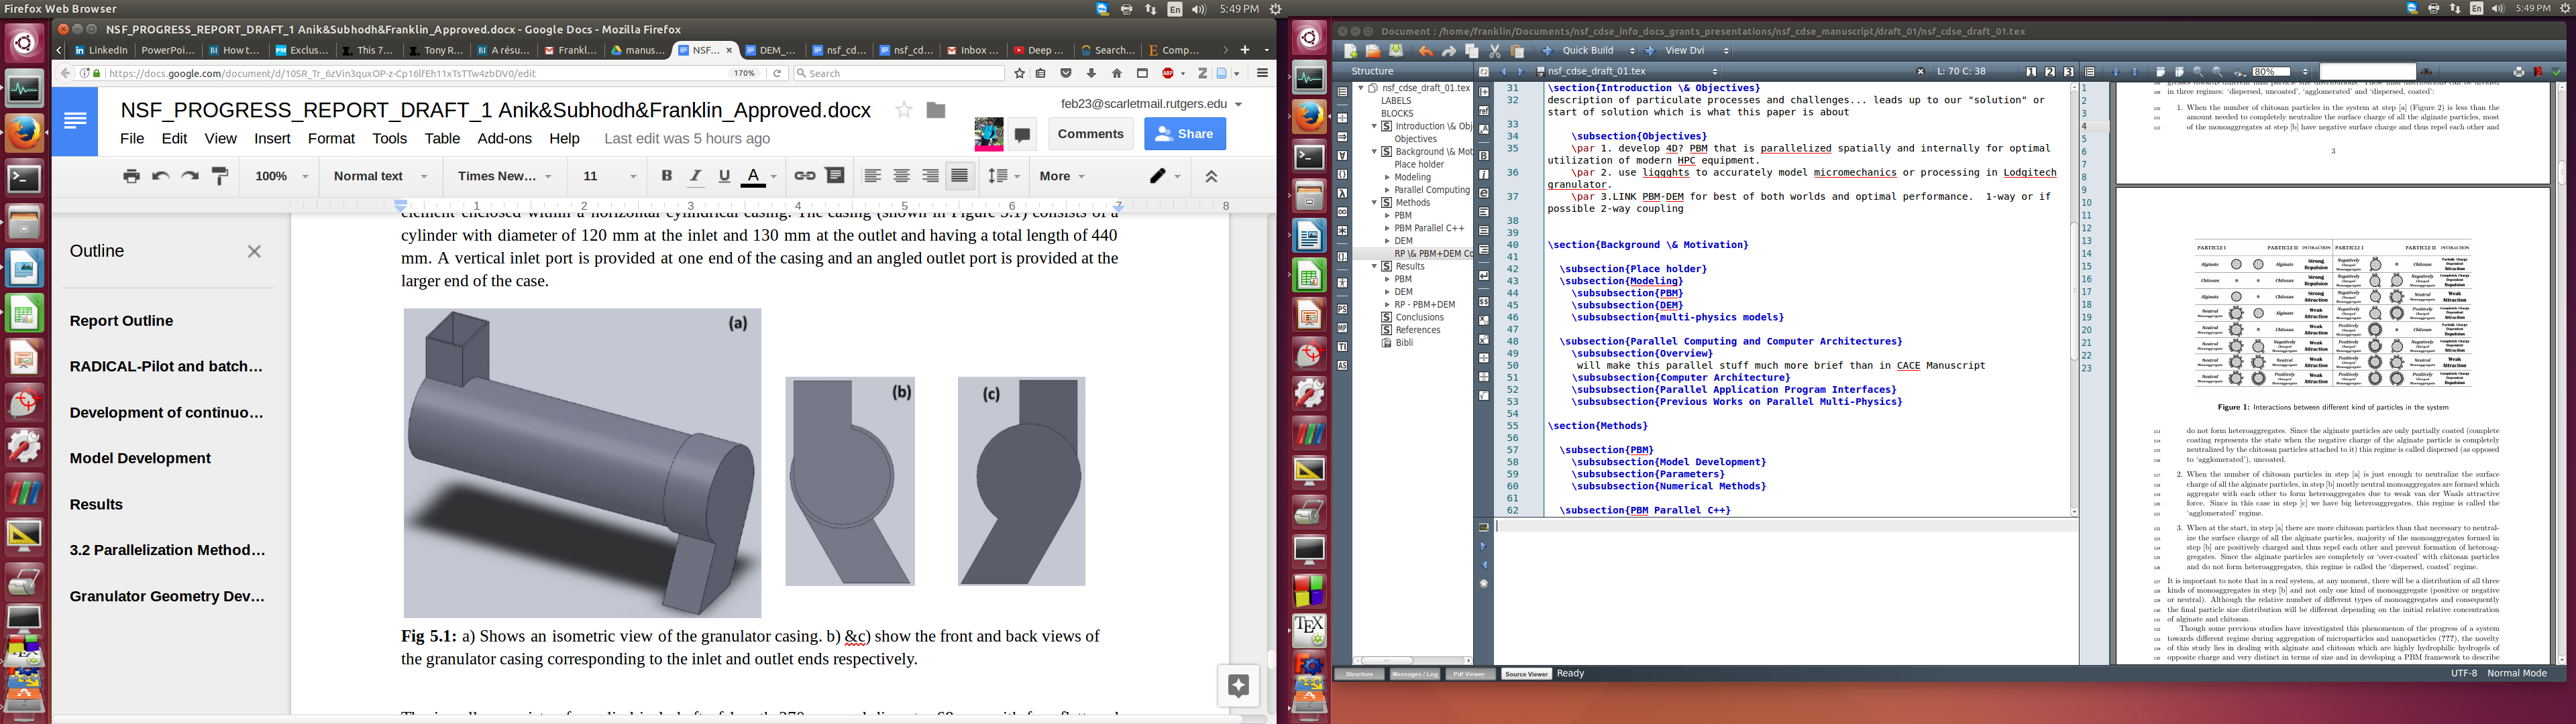
\includegraphics[scale=0.1]{mthds_dem_charles_fig5pt01_gran_shell}
	      \caption{ a) Shows an isometric view of the granulator casing. b) and c) show the front and back views of the granulator casing corresponding to the inlet and outlet ends respectively.}
	      %\caption{hello yuktesh}
	      \label{fig:mthdsDemCharlesGranShell}
	      \end{figure}
	   
	    \par  The impeller consists of a cylindrical shaft of length 370 mm and diameter 68 mm with four flattened sides 15 mm wide running along the axis. The blades are placed on these flattened sides as shown in figure \ref{fig:mthds_dem_charles_impeller}. There are three different blade elements on the shaft (figure \ref{fig:mthds_dem_charles_impeller}). At the granulator inlet, there are 4 paddle shaped feed elements following which there are 20 tear drop shaped shearing elements  and finally 4 trapezoidal blades near the exit. All these elements are placed in a spiral configuration. The final configuration of the granulator is shown in figure \ref{fig:mthds_dem_charles_fig5pt3and4_blades_n_isometric}.
	
	      \begin{figure}[H]
	      \centering
	      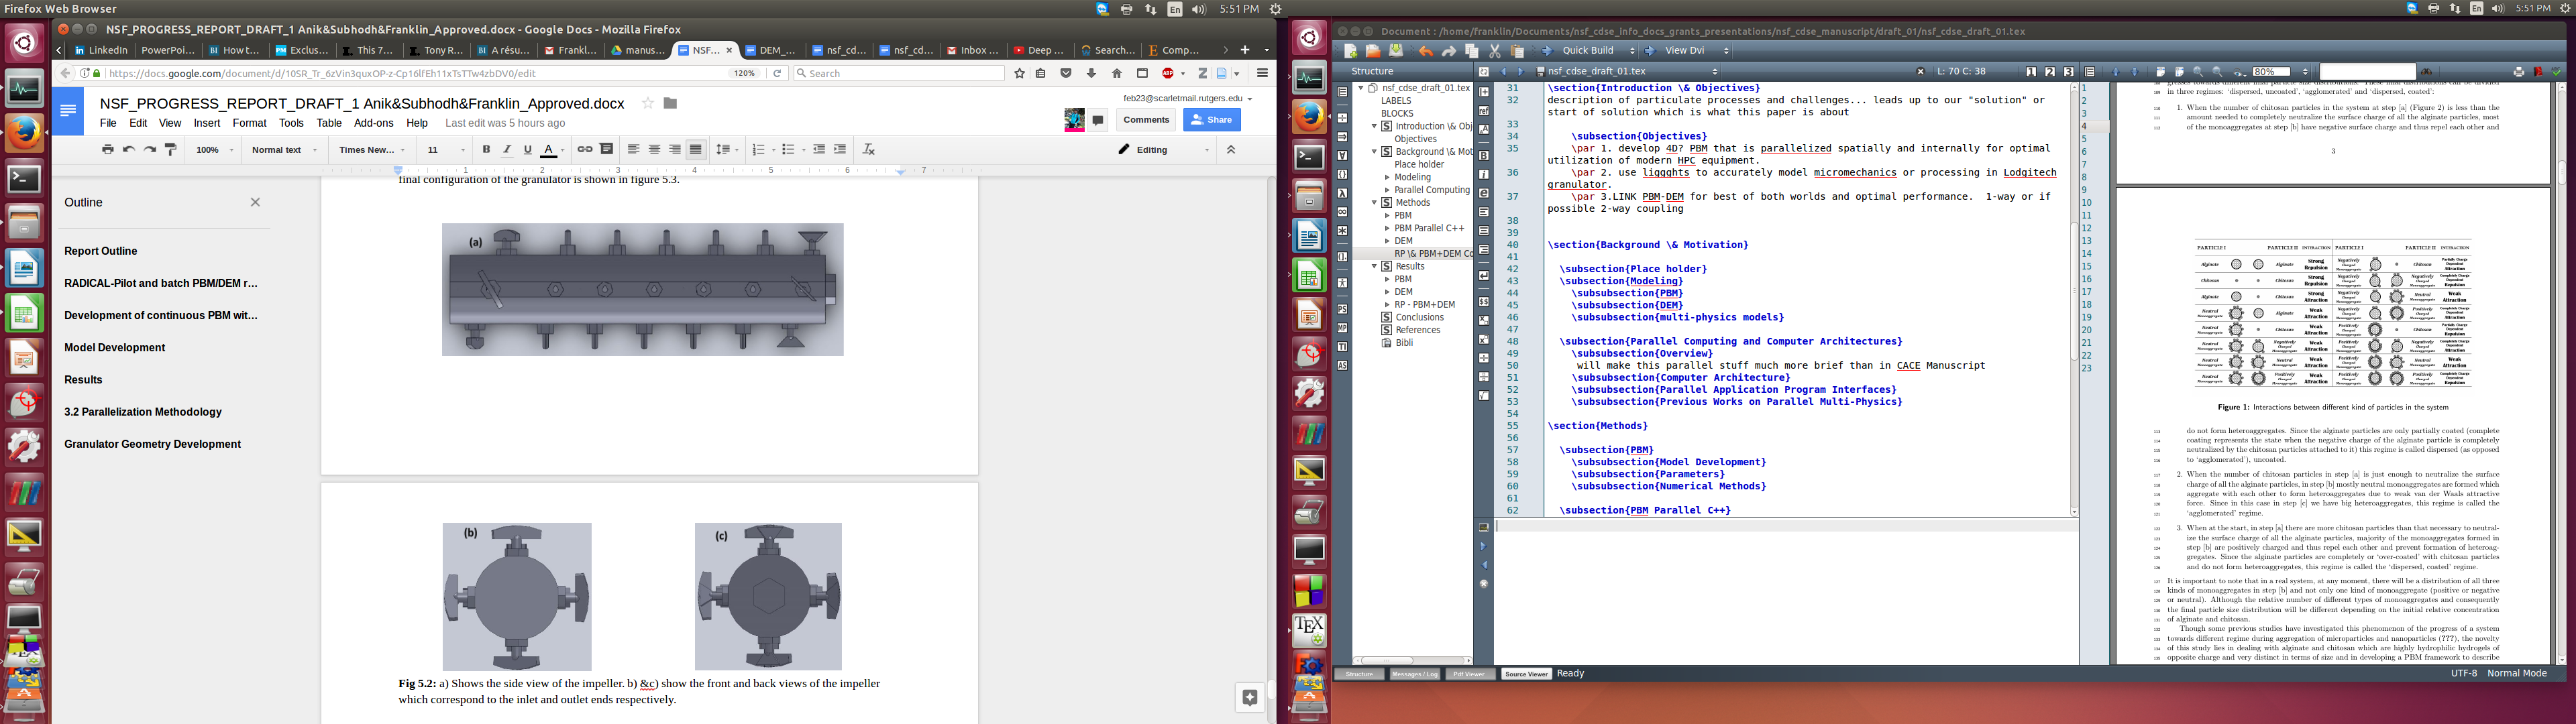
\includegraphics[scale=0.1]{mthds_dem_charles_fig5pt2_impeller}
	      \caption{a) Shows the side view of the impeller. b) and c) show the front and back views of the impeller which correspond to the inlet and outlet ends respectively.}
	      %\caption{hello yuk}
	      \label{fig:mthds_dem_charles_impeller}
	      \end{figure}    
	    
	      \begin{figure}[H]
	      \centering
	      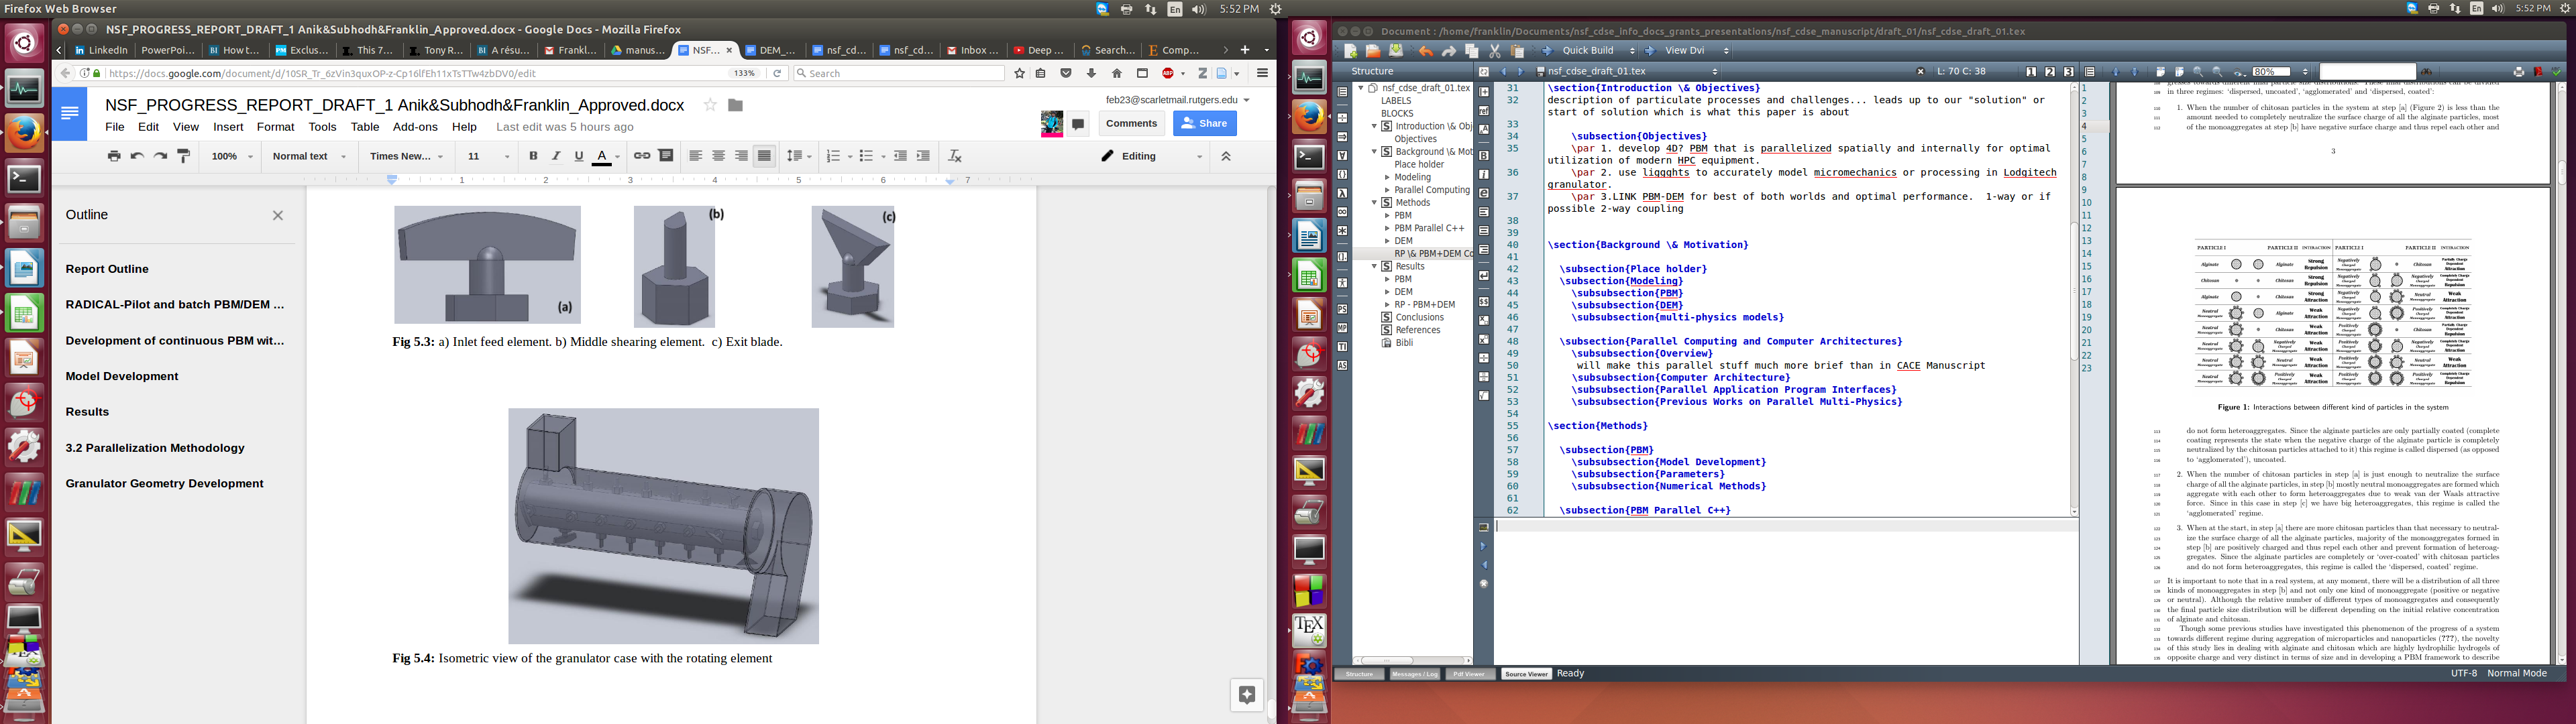
\includegraphics[scale=0.1]{mthds_dem_charles_fig5pt3and4_blades_n_isometric}
	      \caption{a) Inlet feed element. b) Middle shearing element.  c) Exit blade. blah blah Isometric view of the granulator case with the rotating element }
	      %\caption{hello tesh}
	      \label{fig:mthds_dem_charles_fig5pt3and4_blades_n_isometric}
	      \end{figure}     
	    
	
	    
	
	    \subsubsection{Meshing}
	    \par After the geometry was built in solidworks the shell and impeller were exported as \textcolor{cyan}{non-binary} STL files. The coarsest output options(\textcolor{cyan}{include settings even if they were automatic may change from one version to another of SW}) were used to keep the STL files small and simple for faster computations times \textcolor{cyan}{(needs a citation? or is common knowledge?)}. They were also exported not keeping there original coordinates \textcolor{cyan}{(1.too much info 2. what was option in SW for that so I can use that wording)} This resulted in the impeller having x-number-faces and y-number-points with approximately a file size of number KBs. The shell had x-number-faces and y-number-points and approx number KBs.  
	    \par Meshlab was used to align the STL files for importing into LIGGGHTS. No mesh treatments were used on the STLs. 
	    \par The meshes were then imported into LIGGGHTS using the write command (\textcolor{cyan}{more specific command that we actually used?}). This resulted in 50 elements of the impeller file having "highly skewed elements angles < 0.5 deg?" that according to LIGGGHTS would degrade parallel performance. The shell did not have any skewed elements \textcolor{cyan}{(FUTURE SOLUTION? - perhaps we can use the output from liggghts exclusion list to find exact elements of issue. then we can use meshlab to exclude those peices or remesh thos individual pieces into better shapes with less skewed elements. might be better for a letter paper though}
	    
	    \subsubsection{DEM input file settings}
	    \par For the DEM simulations, a input script has to be prepared for LIGGGHTS. The input file consists of various physical parameters of the particles being simulated, command lines for the desired outputs from LIGGGHTS and various dump command which is used for post - processing of the data. 
	    \par Need to add contact models, movement commands, all the start options, 
	    	\begin{table}[!htb]
	\caption{Physical Properties of the particle for the LIGGGHTS input script (Currently a placeholder)} \label{table:mthds_dem_input}
	\begin{center}
	\begin{tabular}{c|c|c|c}
	\hline
	\bf{Parameter} &\bf{Symbol} &\bf{Value} &\bf{Units}\\
	\hline
	Boltzmann constant & $k$ & $1.3806488 \times 10^{-23}$ & $m^2~kg~s^{-2}~K^{-1}$\\
	Charge of electron & $e$ & $1.60217657 \times 10^{-19}$ & $Coulombs$\\
	Avogadro Number & $N_A$ & $6.0221413 \times 10^{23}$ & $-$\\
	Hamaker constant & $A_H$ & $3 \times 10^{-21}$ & $J$\\
	Hydration force constant & $F_0$ & $10^{-2}$ & $N~m^{-1}$\\
	Temperature of the medium & $T$ & $298$ & $K$\\
	Viscosity of the medium & $\mu$ & $0.8999 \times 10^{-3}$ & $Pa.s$\\
	Permittivity of the medium & $\epsilon_0 \epsilon_r$ & $6.93\times 10^{-10}$ & $C^2~N^{-1}~m^{-2}$ \\
	Valence of ions in medium & $z$ & $1$ & $-$\\
	Bulk concentration of ions in medium & $C^b$ & $1 \times 10^{-2}$ & $kg~m^{-3}$\\
	Debye length & $\frac{1}{\kappa} $ & $1.3581 \times 10^{-7}$ & $m$\\
	Decay length & $\delta_0$ & $6 \times 10^{-10}$ & $m$\\
	Density of alginate & $\rho_{Alginate}$ & $1050$ & $kg~m^{-3}$ \\
	Density of chitosan & $\rho_{Chitosan}$ & $1000$ & $kg~m^{-3}$ \\
	Surface potential of alginate & $\Psi_{Alginate}$ & $-46 \times 10^{-3}$ & $Volts$\\
	Surface potential of chitosan & $\Psi_{Chitosan}$ & $56 \times 10^{-3}$ & $Volts$\\
	Volume of the system & $V$ & $10\times10^{-6}$ & $m^3$\\
	Volume of the smallest alginate bin & $a_1$ & $1.5 \times 10^{-17}$ & $m^{3}$\\
	Volume of the smallest chitosan bin & $c_1$ & $0.3 \times 10^{-17}$ & $m^{3}$ \\
	Aggregation kernel constant & $K_0$ & $5 \times 10^{9}$ & $-$\\
	Simulated Process Time & $t$ & $10$ & $s$\\
	Simulation Time-Step & $dt$ & $0.01$ & $s$\\
	\hline
	\end{tabular}
	\end{center}
	\end{table}

	    \subsubsection{DEM Post data analysis}
	    \par matlab script to check for constant flow/ steady state talk about the methods it uses etc? 
	    
	    \par matlab script to check for particles leaving etc make sure all good 
	     
	    
	  \subsection{PBM}
	    \subsubsection{Model Development}
	    \par The main PBM equation developed for this work can be expressed as shown below:
	    \begin{align}
	    \frac{d}{dt}F(s_1,s_2,x)=\Re_{agg}(s_1,s_2,x)+R_{break}(s_1,s_2,x)+\dot{F}_{in}(s_1,s_2,x)-\dot{F}_{out}(s_1,s_2,x)
	    \label{eqn:mthds_pbm_overall} 
	    \end{align}
	    \par \textcolor{red}{citation?}    
	    
	    \par where, $F(s_1,s_2,x)$ is the number of particles with an API volume of $s_1$ and an excipient volume of $s_2$ in the spatial compartment $x$. The rate of change of number of particles with time in different size classes depend on the rate of aggregation $\Re_{agg}(s_1,s_2,x)$ and the rate of breakage $\Re_{break}(s_1,s_2,x)$. Also, the rate of particles coming into, $F_{in}(s_1,s_2,x)$ and going out, $F_{out}(s_1,s_2,x)$ of the spatial compartment due to particle transfer affect the number of particles in different size classes. 
	The rate of change of liquid volume is calculated using the equation: 
	
	    \begin{align}
	    \frac{d}{dt}F(s_1,s_2,x)l(s_1,s_2,x)=& \Re_{liq,agg}(s_1,s_2,x)+\Re_{liq,break}(s_1,s_2,x)+\dot{F}_{in}(s_1,s_2,x)l_{in}(s_1,s_2,x)\notag\\
	    &-\dot{F}_{out}(s_1,s_2,x)l_{out}(s_1,s_2,x)+F(s_1,s_2,x)\dot{l}_{add}(s_1,s_2,x)
	    \end{align}
	    
	    \par where, $l(s_1,s_2,x)$ is the amount of liquid volume in each particle with API volume of $s_1$ and excipient volume of $s_2$ in the spatial compartment $x$. $\Re_{liq,agg}(s_1,s_2,x)$ and $\Re_{liq,break}(s_1,s_2,x)$ are respectively the rates of liquid transferred between size classed due to aggregation and breakage. $l_{in}(s_1,s_2,x)$ and $l_{out}(s_1,s_2,x)$ are respectively the liquid volumes of the particles coming in and going out of the spatial compartment. $l_{add}(s_1,s_2,x)$ is the volume of liquid acquired by each particle in the compartment at every time step due to external liquid addition. 
	    \par Similarly, the rate of change of gas volume is calculated using the following equation: 
	    \begin{align}
	    \frac{d}{dt}F(s_1,s_2,x)g(s_1,s_2,x)=& \Re_{gas,agg}(s_1,s_2,x)+\Re_{gas,break}(s_1,s_2,x)+\dot{F}_{in}(s_1,s_2,x)g_{in}(s_1,s_2,x)\notag\\
	    &-\dot{F}_{out}(s_1,s_2,x)g_{out}(s_1,s_2,x)+F(s_1,s_2,x)\dot{g}_{cons}(s_1,s_2,x)
	    \end{align}
	    \par \textcolor{red}{citation?}
	    
	    \par where, $g(s_1,s_2,x)$ is the gas volume of each particle with API volume of $s_1$ and excipient volume of $s_2$ in the spatial compartment $x$. $\Re_{gas,agg}(s_1,s_2,x)$ and $\Re_{gas,break}(s_1,s_2,x)$ are respectively the rates of gas transferred between size classed due to aggregation and breakage. $g_{in}(s_1,s_2,x)$ and $g_{out}(s_1,s_2,x)$ are respectively the gas volume of the particles entering and leaving the spatial compartment. $g_{cons}(s_1,s_2,x)$ is the volume of gas coming out of each particle in the compartment at every time-step due to consolidation of the particles. 
	    \par The rate of aggregation, $\Re_{agg}(s_1,s_2,x)$ in Equation \ref{eqn:mthds_pbm_overall} is calculated as  
	     \begin{align}
	     \Re_{agg}(s_1,s_2,x)=& \frac{1}{2}\int _0^{s_1} \int_0^{s_2} \beta(s_1',s_2',s_1-s_1',s_2-s_2',x)F(s_1',s_2',x)F(s_1-s_1',s_2-s_2',x)ds_1'ds_2'\notag\\ 
	     &- F(s_1,s_2,x)\int _0^{s_{max_1}-s_1} \int_0^{s_{max_2}-s_2} \beta(s_1,s_2,s_1',s_2',x)F(s_1',s_2',x)ds_1'ds_2'
	     \end{align}
	     \par \textcolor{red}{citation?}
	     
	    \par where, the aggregation kernel, $\beta(s_1,s_2, s_1',s_2',x)$ is expressed as –
	    \begin{align}
	    \beta(s_1,s_2,s_1',s_2',x) = & \beta_o*(V(s_1,s_2,x)+V(s_1',s_2',x))^{\gamma}*(c(s_1,s_2,x)\notag\\
	    &+c(s_1',s_2',x))^{\alpha}\left(1-\frac{(c(s_1,s_2,x)+c(s_1',s_2',x))^{\delta}}{2}\right)^{\alpha}
	    \label{eqn:mthds_pbm_beta_kernal}
	    \end{align}
	    \par \textcolor{red}{citation?}
	    
	    \par where, $\beta_o$,  $\alpha$ , $\delta$ and $\gamma$ are aggregation rate constants, $V(s_1,s_2, x)$ and $V(s_1',s_2',x)$ are the volumes of the aggregating particles. $c(s_1,s_2, x)$ and $c(s_1',s_2',x)$ are the external liquid fraction of the aggregating particles. 
	    \par Similarly, the breakage rate is expressed as-
	
	    \begin{align}
	    \Re_{break}(s_1,s_2,x) = \int_0^{s_{max_1}} \int_0^{s_{max_2}} K_{break}(s_1',s_2',x)F(s_1',s_2',x)ds_1'ds_2' - K_{break}(s_1,s_2,x)F(s_1,s_2,x)
	    \end{align}
	    \par \textcolor{red}{citation?}
	    
	    \par where, the breakage kernel $K_{break}(s_1,s_2,x)$ is formulated as – 
	    
	    \begin{align}
	    K_{break}(s_1,s_2,x)=\left(\frac{4}{15\pi}\right)^{(\frac{1}{2})}G_{shear}exp\left(-\frac{B}{R(s_1,s_2,x)}\right)
	    \end{align}
	    \par \textcolor{red}{citation?}
	
	      \par where, $G_{shear}$ is the shear rate exerted by the impeller on the granules. $R(s_1,s_2,x)$ is the radius of the granule that breaks and $B$ is the breakage kernel constant. $G_shear$ is calculated as $\frac{\nu_{impeller}*D_{impeller}*PI}{60}$ where $\nu_{impeller}$ and $D_{impeller}$ are respectively the rotational speed and diameter of the impeller.
	      \par The rate of increase of liquid volume of one particle, $\dot{l}_{add}(s_1,s_2,x)$ is expressed as $\frac{(s_1+s_2)(\dot{m}_{spray}(1-c_{binder})-\dot{m}_evap)}{m_{solid}(x)}$ where, $(s_1+s_2)$  is the total solid volume of the particle; $\dot{m}_spray$ is the rate of external liquid addition, $c_{binder}$ is the concentration of binder in the external liquid (which is assumed to be zero in this case as pure liquid is added); $\dot{m}_{evap}$ is the rate of evaporation of liquid from the system (which is also assumed to be zero in this case) and $m_{solid}$ is the total amount of solid present in the compartment.
	      \par The rate of decrease in gas volume per particle due to consolidation is calculated using the following expression: 
	      
	      \begin{align}
	      \dot{g}_{cons}(s_1,s_2,x)=c*(\nu_{impeller})^{\omega}*V(s_1,s_2,x)\frac{(1-\epsilon_{min})}{s} [g(s_1,s_2,x)+l(s_1,s_2,x) -(s_1+s_2)\frac{\epsilon_{min}}{1-\epsilon_{min}}]
	      \end{align}          
	    
	    \par where, $c$ and $\omega$ are the consolidation constants; $v_{impeller}$ is the impeller rotational speed; $V(s_1,s_2,x)$ is the volume of particle, $\epsilon_{min}$ is the minimum porosity; $g(s_1,s_2,x)$ and $l(s_1,s_2,x)$ are respectively the gas and liquid volume of the particle.
	  
	    \par Particle transfer rate, $F_{out}(s_1,s_2,x)$ in Equation \ref{eqn:mthds_pbm_overall} is calculated as $F(s_1,s_2,x)*\frac{\nu_{compartment(x)}*dt}{d_{compartment}}$ where, $\nu_{compartment(x)}$ and $d_{compartment}$ are respectively the average velocity of particles in compartment $x$ and the distance between the mid-points of two adjacent compartment, which is the distance particles have to travel to move to the next spatial compartment. $dt$ is the time-step.
	The values of various parameters used in the model are provided in Table \ref{table:mthds_pbm_parameters}.
	
	\begin{table}[!htb]
	\caption{Parameters for PBM from Anik's hetero. agg. paper. currently place holder} \label{table:mthds_pbm_parameters}
	\begin{center}
	\begin{tabular}{c|c|c|c}
	\hline
	\bf{Parameter} &\bf{Symbol} &\bf{Value} &\bf{Units}\\
	\hline
	Boltzmann constant & $k$ & $1.3806488 \times 10^{-23}$ & $m^2~kg~s^{-2}~K^{-1}$\\
	Charge of electron & $e$ & $1.60217657 \times 10^{-19}$ & $Coulombs$\\
	Avogadro Number & $N_A$ & $6.0221413 \times 10^{23}$ & $-$\\
	Hamaker constant & $A_H$ & $3 \times 10^{-21}$ & $J$\\
	Hydration force constant & $F_0$ & $10^{-2}$ & $N~m^{-1}$\\
	Temperature of the medium & $T$ & $298$ & $K$\\
	Viscosity of the medium & $\mu$ & $0.8999 \times 10^{-3}$ & $Pa.s$\\
	Permittivity of the medium & $\epsilon_0 \epsilon_r$ & $6.93\times 10^{-10}$ & $C^2~N^{-1}~m^{-2}$ \\
	Valence of ions in medium & $z$ & $1$ & $-$\\
	Bulk concentration of ions in medium & $C^b$ & $1 \times 10^{-2}$ & $kg~m^{-3}$\\
	Debye length & $\frac{1}{\kappa} $ & $1.3581 \times 10^{-7}$ & $m$\\
	Decay length & $\delta_0$ & $6 \times 10^{-10}$ & $m$\\
	Density of alginate & $\rho_{Alginate}$ & $1050$ & $kg~m^{-3}$ \\
	Density of chitosan & $\rho_{Chitosan}$ & $1000$ & $kg~m^{-3}$ \\
	Surface potential of alginate & $\Psi_{Alginate}$ & $-46 \times 10^{-3}$ & $Volts$\\
	Surface potential of chitosan & $\Psi_{Chitosan}$ & $56 \times 10^{-3}$ & $Volts$\\
	Volume of the system & $V$ & $10\times10^{-6}$ & $m^3$\\
	Volume of the smallest alginate bin & $a_1$ & $1.5 \times 10^{-17}$ & $m^{3}$\\
	Volume of the smallest chitosan bin & $c_1$ & $0.3 \times 10^{-17}$ & $m^{3}$ \\
	Aggregation kernel constant & $K_0$ & $5 \times 10^{9}$ & $-$\\
	Simulated Process Time & $t$ & $10$ & $s$\\
	Simulation Time-Step & $dt$ & $0.01$ & $s$\\
	\hline
	\end{tabular}
	\end{center}
	\end{table}
	
	    \subsubsection{Parameters}
	    
	    
	  \subsection{PBM Parallel C++}
	    \subsubsection{Discretization \& Parallelizing PBM}
	    \par To solve the PBM numerically it was discretized using a finite element method type solution. To obtain the most optimal parallel performance, when solving the PBM, work loads were distributed in a manner which took into account the shared memory and distributed memory aspects of the clusters the PBM was being run on. To parallelize the model in a why which could use shared and distributed methods of OMP and MPI were used. 
	    \par One MPI process was used per CPU socket and one OMP process was used per CPU core, as authors (\cite{Bettencourt2017}) found it resulted in the best performance. MPI was used for message passing from one node to another while OMP was used for calculations on each node that could be efficiently solved using a shared memory system \textcolor{cyan}{i.e. calculations were inter-dependent but could be computed simultaneously.} 
	    \par Pseudo code is presented below illustrating how the calculations are distributed and carried out during the simulation. For each time step the MPI processes are made responsible for a specific chunk of the spatial compartments. Then each OMP thread, inside of each MPI process, is allocated to one of the cores of the the multi-core CPU the MPI process is bound too. The OMP processes divide up and compute $\Re_{agg}$ and $\Re_{brk}$. (\textcolor{cyan}{include more detail about how they do it? last paper reviewer complained that could not understand figure by JUST reading what I wrote about it in meat of paper}) 
	    \par After $\Re_{agg}$ and $\Re_{brk}$ are calculated the MPI processes calculate the new PSD value for their chunk at that specific time step, $F_{t,c}$. The slave processes send their $F_{t,c}$ to the master processes which collects them into the complete $F_{t,all}$. The master process then broadcasts the $F_{t,all}$ value to all slave processes. 	
	    \par A crucial feature of the PBM is that the current PSD ($F_{t,all}$) value is used to compute a new time step size for the next iteration. This means all of the MPI processes need to have the same dynamic time step size at each iteration for the calculations to be properly carried out in parallel. Since the completely updated $F_{t,all}$ value is shared before calculating a new time step each process will have the same $F_{t,all}$ value. As a result each process calculates the same size for the new time step. 
	\textcolor{cyan}{ Did not include the liquid and gas PBMs in this but hoping they will be some what assumed? Also the Ragg omp distributed work is an a}
	\textcolor{red}{what about private OMP vars specified that has impact on how model is solved etc. Should look into this. might change based on locking/blocking tests that need to be implemented still.}   
	
	  \begin{algorithm*}[!h]
	   \caption{Pseudo code}
	    \begin{algorithmic}[*]
	     \While{ $t<t_{final}$ }
	      \par // the spatial domain is divided into equal chunks (with in 1 bin size)
	      \par // each MPI process is assigned on chunk of spatial domain shown as $c_{low}$ to $c_{up}$ 
	      \par // sum all $c_{low_i}$ to $c_{up_i}$ is = to [0,numCompartments]
	  
	        \For{each MPI processes} $c = c_{low_i}$ to $c_{up_i}$
		  	\par   // each MPI process is further divided with OMP to take advantage of multi-core CPU
			\par   // each OMP process is allocated to a single compute core
			\par   // $\Re$ integrals $(i1)$ $\int_{0}^{s_2}$, $(i2)$ $\int_{0}^{s_{max_2}-s_2}$, and $(i3)$ $\int_{0}^{s_{max_2}-s_2}$ are divided into smaller integrals
			\par  // $\int_{i_1low_n}^{i_1up_n}$, $\int_{i_2low_n}^{i_2up_n}$, and $\int_{i_3low_n}^{i_3up_n}$ which are solved by the "n" OMP processes
	        \par   // allocated to that MPI process (CPU)
	          \For{ each OMP process}
	
	     \begin{align}
	     \Re_{agg}(s_1,s_2,c)=& \frac{1}{2}\int_{0}^{s_{1}} \int_{i_1low_n}^{i_1up_n} \beta(s_1',s_2',s_1-s_1',s_2-s_2',c)F(s_1',s_2',c)F(s_1-s_1',s_2-s_2',c)ds_1'ds_2'\notag\\ 
	     &- F(s_1,s_2,c)\int _{0}^{s_{max_1}-s_1} \int_{i_2low_n}^{i_2up_n} \beta(s_1,s_2,s_1',s_2',c)F(s_1',s_2',c)ds_1'ds_2'\notag
	     \end{align}
	     \begin{align*}
	    \Re_{break}(s_1,s_2,c) = \int_{0}^{s_{max_1}} \int_{i_3low_n}^{i_3up_n} K_{break}(s_1',s_2',c)F(s_1',s_2',c)ds_1'ds_2' - K_{break}(s_1,s_2,c)F(s_1,s_2,c)
	     \end{align*}
	         \EndFor 
	     \begin{align*}
	   F_{t,c} &= \frac{\Delta F(s_1,s_2,c)}{\Delta t}\Delta t  + F(s_1,s_2,c)_{t-1}\\
	                  &=   (\Re_{agg}(s_1,s_2,c)+\Re_{break}(s_1,s_2,c)+\dot{F}_{in}(s_1,s_2,c)-\dot{F}_{out}(s_1,s_2,c))\Delta t + F(s_1,s_2,c)_{t-1}
	     \end{align*}
	
	        \EndFor
	     \State MPI Send $F_{t,c}$ to Master MPI process
	     \State MPI Recv $F_{t,c}$ from MPI all slave processes
	     \State Master consolidate all $F_{t,c}$ chunks into a complete $F_{t,all}$
	     \State Master does inter-bin particle transfers (updates $F_{t,all}$)
	     \State MPI Bcast $F_{t,all}$ to all slave processes
	     \State $t_{new} = t + timestep$
	        
	     \EndWhile   
	
	\end{algorithmic}
	\end{algorithm*}   
	    
	  
	  \subsection{RP \& PBM+DEM Communication}
	
	
	  
	\section{Results}
	  \subsection{PBM}
	    \subsubsection{PBM Validation}
	      
	
	      \begin{figure}[H]
	      \centering
	      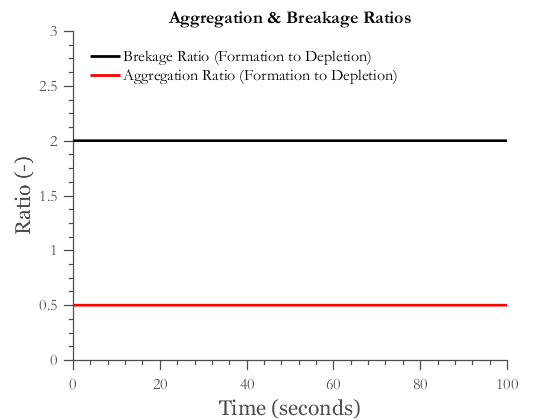
\includegraphics[scale=0.5]{rslts_anik_pbm_ratios}
	      \caption{Ratio of formation-to-depletion through aggregation and breakage over time. Breakage ratio of 2 and aggregation ratio of 0.5 indicate mass conservation in the model. \textcolor{red}{NOTE DID NOT HAVE .fig file for this figure so it is in as JPG will need to replace} }
	      %\caption{hello tesh}
	      \label{fig:rslts_anik_pbm_ratios}
	      \end{figure}
	     
	     \par The ratio between the number of particles formed due to aggregation and the number of particles depleted due to aggregation and the ratio of the number of particles formed due to breakage to the number of particles depleted due to breakage are plotted. In aggregation two particles agglomerate to form one particle and in breakage one particle breaks to form two particles. So, these ratios are expected to be 0.5 and 2 respectively. As can be seen from Figure \ref{fig:rslts_anik_pbm_ratios}, these ratios are accurate confirming that mass is conserved accurately in the model.
	\par The granulator was divided into 3 compartments spatially and the total volume, solid volume and pore volume and the median diameter $d_50$ in each compartment were plotted to study the granulation behaviour and are shown in Figure \ref{fig:rslts_anik_pbm_total_vol_solid_pore_d50}. 
	\par It can be seen from Figure \ref{fig:rslts_anik_pbm_total_vol} that the total volume starts to increase first in compartment 1 followed by compartment 2 and then compartment 3. This happens as gradually particles entering compartment 1 moves to the other compartment due to particle transfer from compartment 1 to compartment 2 and then compartment 3. In Figure \ref{fig:rslts_anik_pbm_total_solid_vol} it is observed that the solid volume similar to the total volume increases first in compartment 1 and last in compartment 3. The solid volume becomes constant and equal in all the compartments at around 30-50 seconds and steady state is reached when the rate of particle volume being transported through the compartments and leaving the system is equal to the rate of particles entering the system. Although, as seen in Figure \ref{fig:rslts_anik_pbm_total_pore_vol} the pore volume which is the sum of the gas and the liquid volume is highest in compartment 3 and lowest in compartment 1. This happens due to the external liquid addition to the system. As the particles move from compartment 1 to compartment 3, they gradually acquire a higher amount liquid, thereby increasing the pore volume. In Figure \ref{fig:rslts_anik_pbm_d50}, the $D_50$ is seen to be increasing from compartment 1 to 3. This happens because of the size enlargement of large particles coming in from the previous compartment because of the external liquid added to each compartment and a longer residence time in the granulator. 
	
	\begin{figure}[H]
	    \centering
	    \begin{subfigure}[b]{0.45\textwidth}
	        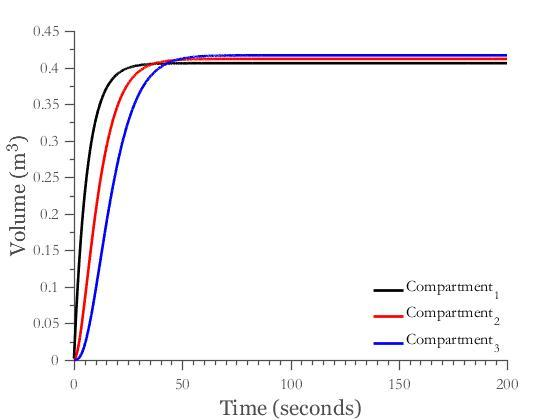
\includegraphics[width=\textwidth]{rslts_anik_pbm_total_vol}
	        \caption{Total volume in all compartments}
	        \label{fig:rslts_anik_pbm_total_vol}
	    \end{subfigure}
	    ~ %add desired spacing between images, e. g. ~, \quad, \qquad, \hfill etc. 
	      %(or a blank line to force the subfigure onto a new line)
	    \begin{subfigure}[b]{0.45\textwidth} 
	        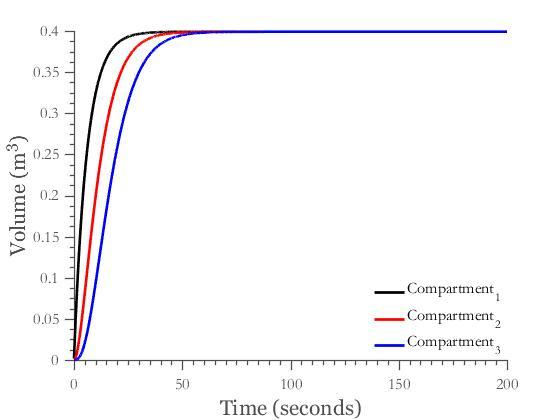
\includegraphics[width=\textwidth]{rslts_anik_pbm_total_solid_vol}
	        \caption{Total solid volume in all compartments}
	        \label{fig:rslts_anik_pbm_total_solid_vol}
	    \end{subfigure}
	    ~ %add desired spacing between images, e. g. ~, \quad, \qquad, \hfill etc. 
	    %(or a blank line to force the subfigure onto a new line)
	    
	    \begin{subfigure}[b]{0.45\textwidth}
	        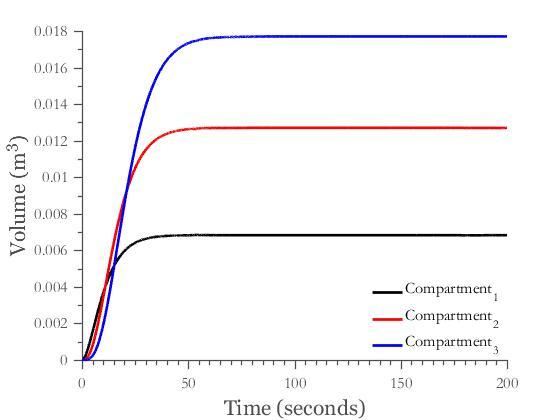
\includegraphics[width=\textwidth]{rslts_anik_pbm_total_pore_vol}
	        \caption{Total pore volume in all compartments}
	        \label{fig:rslts_anik_pbm_total_pore_vol}
	    \end{subfigure}
	    \begin{subfigure}[b]{0.45\textwidth}
	        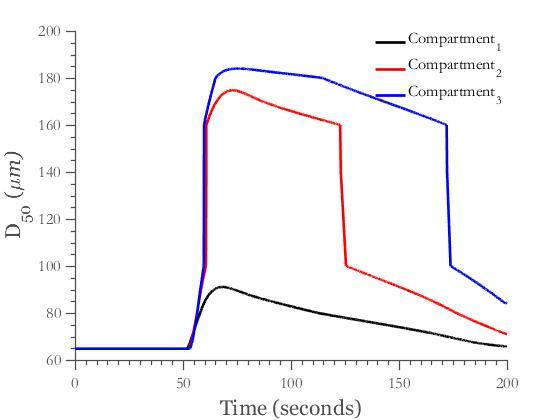
\includegraphics[width=\textwidth]{rslts_anik_pbm_d50}
	        \caption{D$_{50}$ in all compartments}
	        \label{fig:rslts_anik_pbm_d50}
	    \end{subfigure}
	
	    \caption{Volume and D50 in all compartments over time. Volumes become constant as steady state is reached. Median diameter increases and then decreases as bigger particles leave the system and smaller particles occupy that volume.}\label{fig:rslts_anik_pbm_total_vol_solid_pore_d50}
	\end{figure}
	
	
	    \subsubsection{Parallel C++ PBM Validation}
	   \par show PSD or $D_50$ is the same as Matlab or serial PBM
	   \par 1. fig $D_50$ Matlab vs Parallel
	      \begin{figure}[!htb]
	      \centering
	      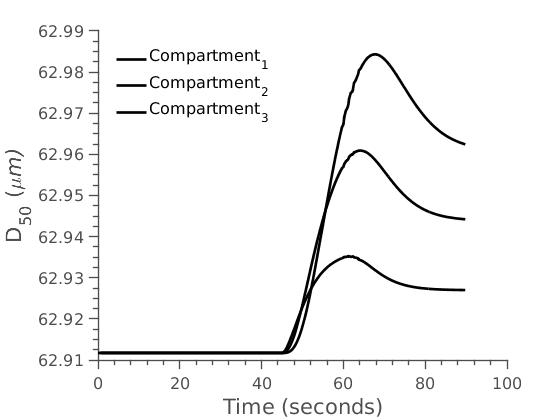
\includegraphics[scale=0.5]{rslts_pbm_d_50_pll_vldtn}
	      \caption{ $D_{50}$ of Matlab PBM vs Parallel PBM}
	      %\caption{hello tesh}
	      \label{fig:rslts_pbm_d_50_vldtn}
	      \end{figure}
	    
	    \subsubsection{Parallel PBM Performance}
	     \par show that RP has minimal impact on performance 
	    \par show that performance is mostly unaffected by RP 
	    \par 1. fig scaling 
	      \begin{figure}[H]
	      \centering
	      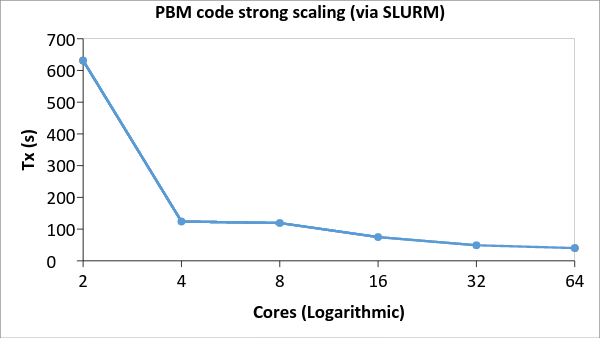
\includegraphics[scale=0.5]{rslts_strong_scale_slurm}
	      \caption{ PBM strong scale slurm}
	      %\caption{hello tesh}
	      \label{fig:rslts_pbm_strong_scale}
	      \end{figure}
	    \par 2. fig scaling w/ RP  
	      \begin{figure}[H]
	      \centering
	      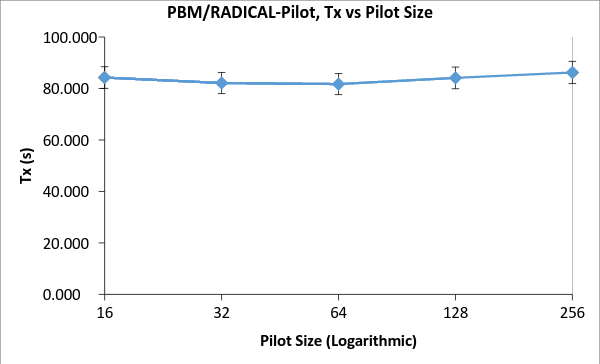
\includegraphics[scale=0.5]{rslts_pbmbyrp_strng}
	      \caption{ PBM strong scale RP}
	      %\caption{hello tesh}
	      \label{fig:rslts_pbmbyrp_strng}
	      \end{figure} 
	      
	    \subsubsection{Parallel PBM Parameter space and Parameter Estimation}
	     \par I. show how effective parallel pbm is for parameter estimation 
	     \par II. Find/ explore ranges of DEM data that PBM can use to find Critical parameters and sensitivities will be useful to us in linking and in picking best DEM parameters to vary and best parameters for PBM+DEM code 
	     \par 1. fig range of some parameters?
	     \par 2. fig range of other pbm parameter ?
	     
	\begin{table}[h]
	%\caption{Parameters used in the Population Balance Model} %\label{table:rslts_pll_pbm}
	%\begin{center}
	%\begin{tabular}{c|c|c|c|c|c|c|c|c}
	%\hline
	%\bf{Cores in Parallel} &\bf{Num. MPI Proc.} &\bf{Threads/ MPI Proc.} &\bf{Wall %Time} &\bf{Speed Up} &\bf{Parallel Effic} &\bf{Pll. Wall Time/ Ser. Wall Time} %&\bf{Gran. Time/ Wall Time} &\bf{Speed Up w.r.t. Matlab}\\
	%\hline
	%$1$   & $1$  & $1$ & $222$ &  $1.00$  & $1.0 $  & $100$  & $246.67$ & $11.57$\\
	%$128$ & $16$ & $8$ & $6$   & $37.000$ & $0.289$ & $2.70$ & $\% 6.67$  & %$428.17$\\
	%\hline
	%\end{tabular}
	%\end{center}
	\end{table}   
	   
	  
	  \subsection{DEM}
	    \subsubsection{DEM Validation and Parameter Space Studies}
	    \par show that DEM is somewhat behaving like a real system
	    \par fig constant flow reached by end of DEM simulation
	      \begin{figure}[H]
	      \centering
	      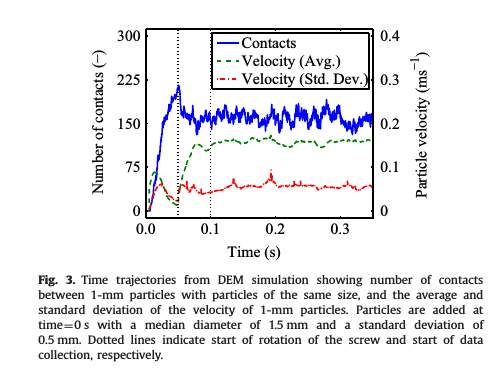
\includegraphics[scale=0.8]{rslts_DEM_time_traj}
	      \caption{  }
	      %\caption{hello tesh}
	      \label{fig:rslts_DEM_time_traj}
	      \end{figure} 
	    \par fig RTD
	    \par show affects of certain parameters on DEM and which ones are most critical to outcomes - will help decide on PBM+DEM parameters to study in later section
	    \par fig vary impeller RPM see how RTD or hold up changes
	    \par fig vary PSD ( range and/or particle sizes) to see how $C_{coll}$ etc will be affected - important for PBM Kernel
	      \begin{figure}[H]
	      \centering
	      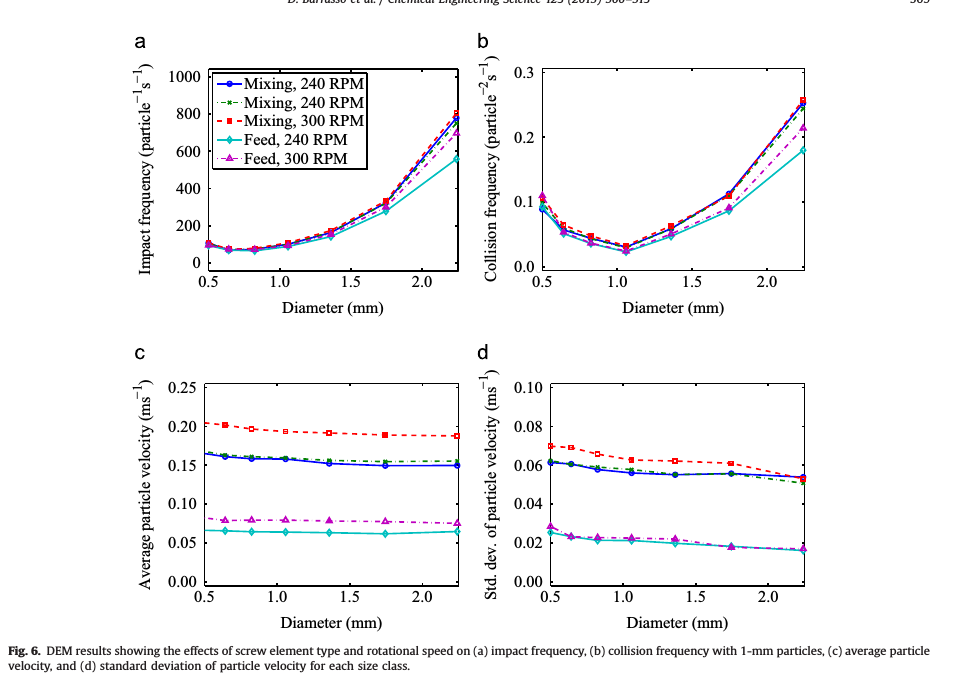
\includegraphics[scale=0.5]{dana_quad_impact_coll_vs_RPM}
	      \caption{ fig showing sensitivity of $C_{coll}$ and etc to RPM}
	      %\caption{hello tesh}
	      \label{fig:rslts_psd_velocity}
	      \end{figure} 
	        
	    \par fig vary impeller RPM see $C_{coll}$ changes
	      \begin{figure}[H]
	      \centering
	      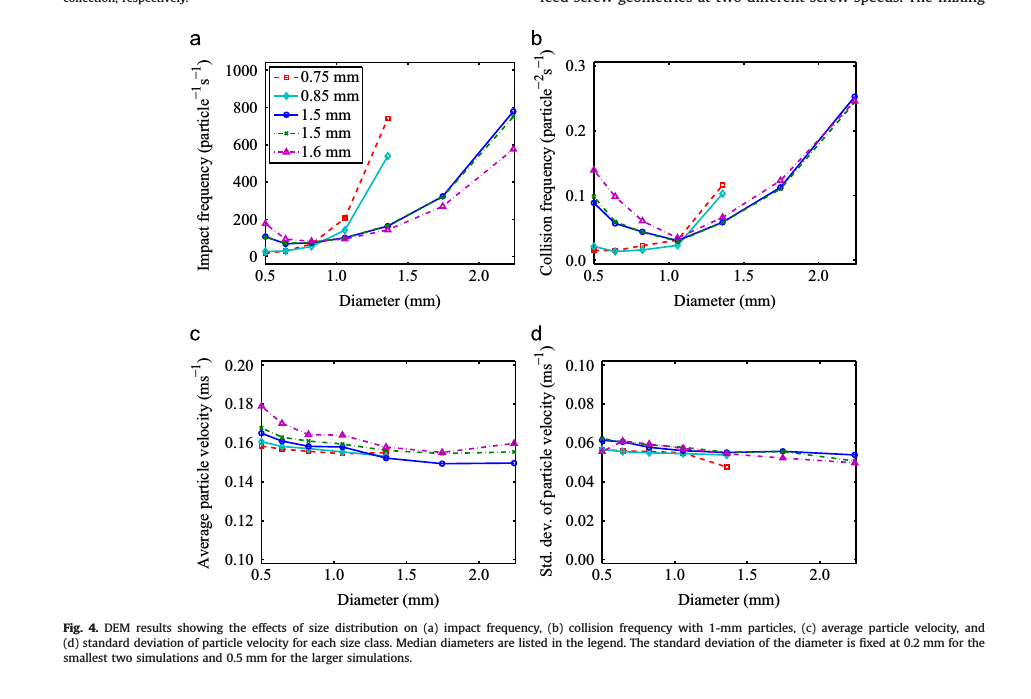
\includegraphics[scale=0.5]{rslts_dem_psd_velocity}
	      \caption{ fig from dana 2015 mechanistic bi-directional}
	      %\caption{hello tesh}
	      \label{fig:rslts_psd_velocity}
	      \end{figure}
	      
	      
	    \subsubsection{DEM Performance}
	    \par show that performance is mostly unaffected by RP 
	    \par 1. fig scaling 
	      \begin{figure}[H]
	      \centering
	      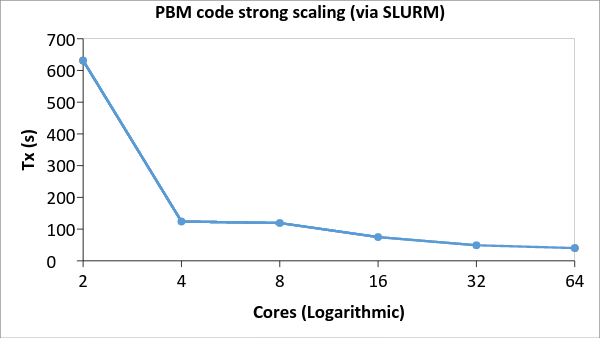
\includegraphics[scale=0.5]{rslts_strong_scale_slurm}
	      \caption{ DEM scale just slurm }
	      %\caption{hello tesh}
	      \label{fig:rslts_DEM_strong_scale}
	      \end{figure}
	    \par 2. fig scaling w/ RP  
	      \begin{figure}[H]
	      \centering
	      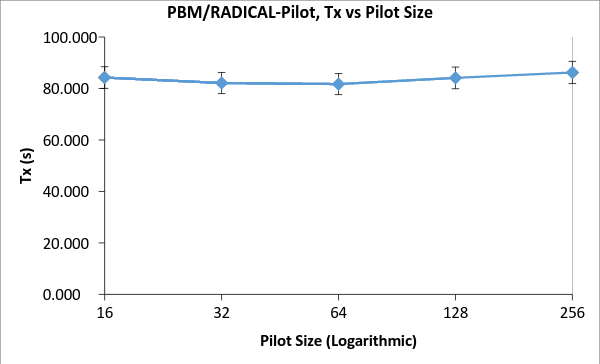
\includegraphics[scale=0.5]{rslts_pbmbyrp_strng}
	      \caption{ DEM scale with RP}
	      %\caption{hello tesh}
	      \label{fig:rslts_dembyRP_strng}
	      \end{figure}
	      
	    %\subsubsection{DEM Parameter Space} 
	 
	    
	  \subsection{PBM+DEM - RP} 
	    \subsubsection{PBM+DEM Validation/Accuracy?}
	   
	    
	    \subsubsection{PBM+DEM Performance}
	    \par strong scaling
	    \par fig PBM + DEM RP strong scaling 
	      \begin{figure}[!htb]
	      \centering
	      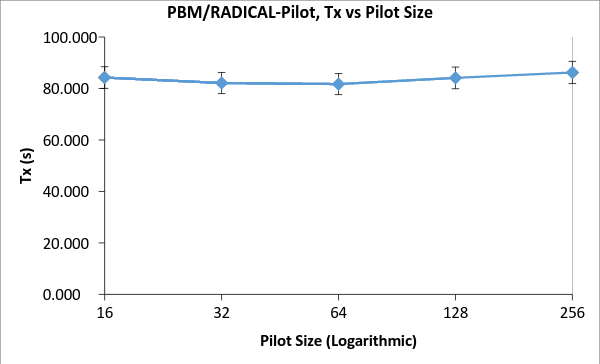
\includegraphics[scale=0.5]{rslts_pbmbyrp_strng}
	      \caption{PBM+DEM scale with RP}
	      %\caption{hello tesh}
	      \label{fig:rslts_dembyRP_strng}
	      \end{figure}
	
	    %\par weak scaling
	    %\par fig PBM + DEM RP weak scaling
	
	
	   \subsubsection{PBM+DEM Parameter studies}
	   \par show how PBM+DEM captures multi-physics as parameters changed. helps validate and support model development. show we have made a useful tool for future work.
	   \par fig 
	      \begin{figure}[H]
	      \centering
	      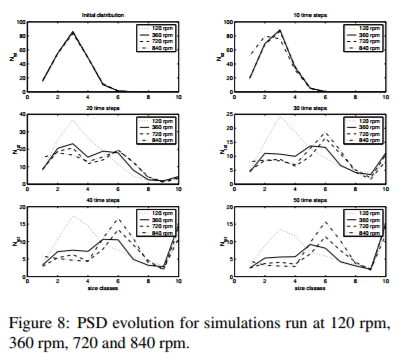
\includegraphics[scale=0.7]{rslts_psd_evo_time}
	      \caption{PBM+DEM scale with RP}
	      %\caption{hello tesh}
	      \label{fig:rslts_psd_evo_time}
	      \end{figure}
	   \par PSD over time for different impeller RPM
	    
	\section{Conclusions}
	
	\section*{References} 
	\bibliographystyle{elsarticle-harv}
	\bibliography{Bibli}
	\end{document}
